\chapter{Resultados y análisis}

\section{Características de las placas sintéticas generadas}
Algunos ejemplos de placas generadas son mostradas en Fig. \ref{fig:ejemplo-placas-sinteticas}

\begin{figure}[H]
    \centering
    % Fila pacheco
    \begin{subfigure}[t]{0.45\textwidth}
        \centering
        
\includegraphics[width=\linewidth]{fig/proy/synthetic_plate_1.png}
        % \caption*{Pacheco - Vista frontal}
    \end{subfigure}
    \hfill
    \begin{subfigure}[t]{0.45\textwidth}
        \centering
        
\includegraphics[width=\linewidth]{fig/proy/synthetic_plate_2.png}
        % \caption*{Pacheco - Vista superior}
    \end{subfigure}
    
	\vspace{1em}
	
	%Fila city
    \begin{subfigure}[t]{0.45\textwidth}
        \centering
        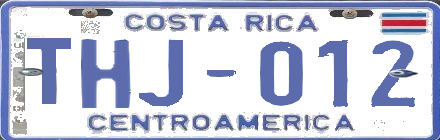
\includegraphics[width=\linewidth]{fig/proy/synthetic_plate_3.png}
        % \caption*{City - Vista frontal}
    \end{subfigure}
	\hfill
    \begin{subfigure}[t]{0.45\textwidth}
        \centering
        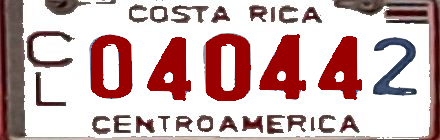
\includegraphics[width=\linewidth]{fig/proy/synthetic_plate_4.png}
        % \caption*{City - Vista superior}
    \end{subfigure}
	
	\vspace{1em}

    % Fila principal
    \begin{subfigure}[t]{0.45\textwidth}
        \centering
        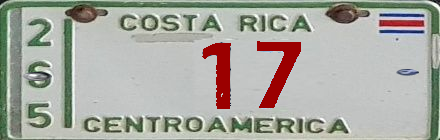
\includegraphics[width=\linewidth]{fig/proy/synthetic_plate_5.png}
        % \caption*{Principal - Vista frontal}
    \end{subfigure}
	\hfill
    \begin{subfigure}[t]{0.45\textwidth}
        \centering
        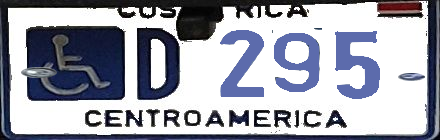
\includegraphics[width=\linewidth]{fig/proy/synthetic_plate_6.png}
        % \caption*{Principal- Vista superior}
    \end{subfigure}
    \caption{Ejemplos de placas sintéticas}
	\label{fig:ejemplo-placas-sinteticas}
\end{figure}

\section{Comparación de desempeño de detección de placas}

\begin{figure}[H]
	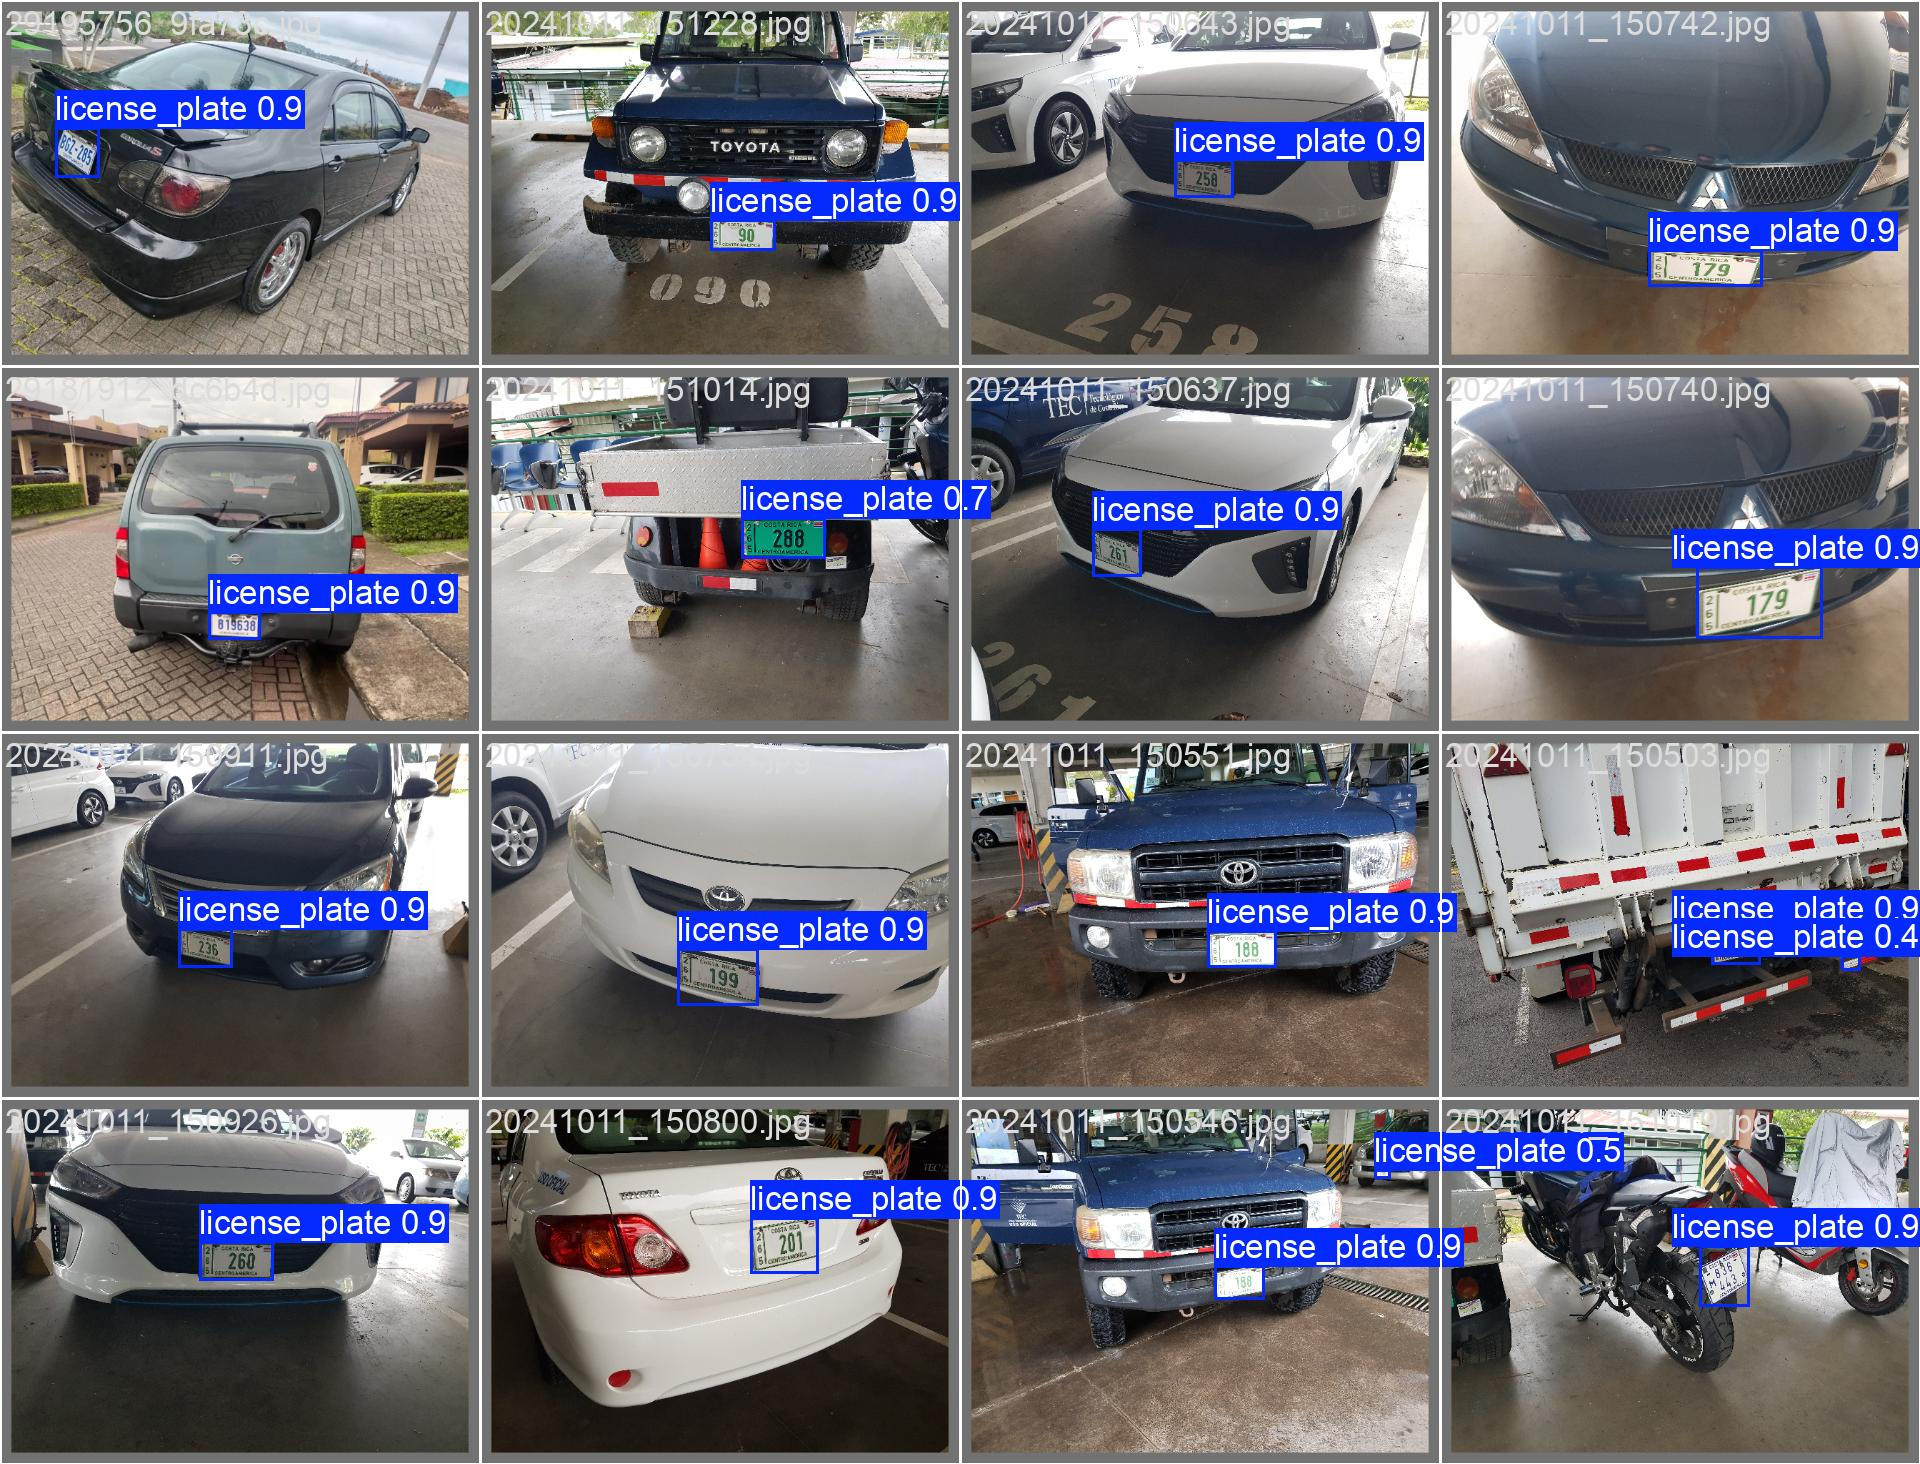
\includegraphics[width=\textwidth]{fig/proy/ejemplo-deteccion-placas.jpg}
	\caption{Ejemplo de detección de placas en imágenes}
	\label{fig:ejemplo-deteccion-placa}
\end{figure}

\begin{figure}[H]
	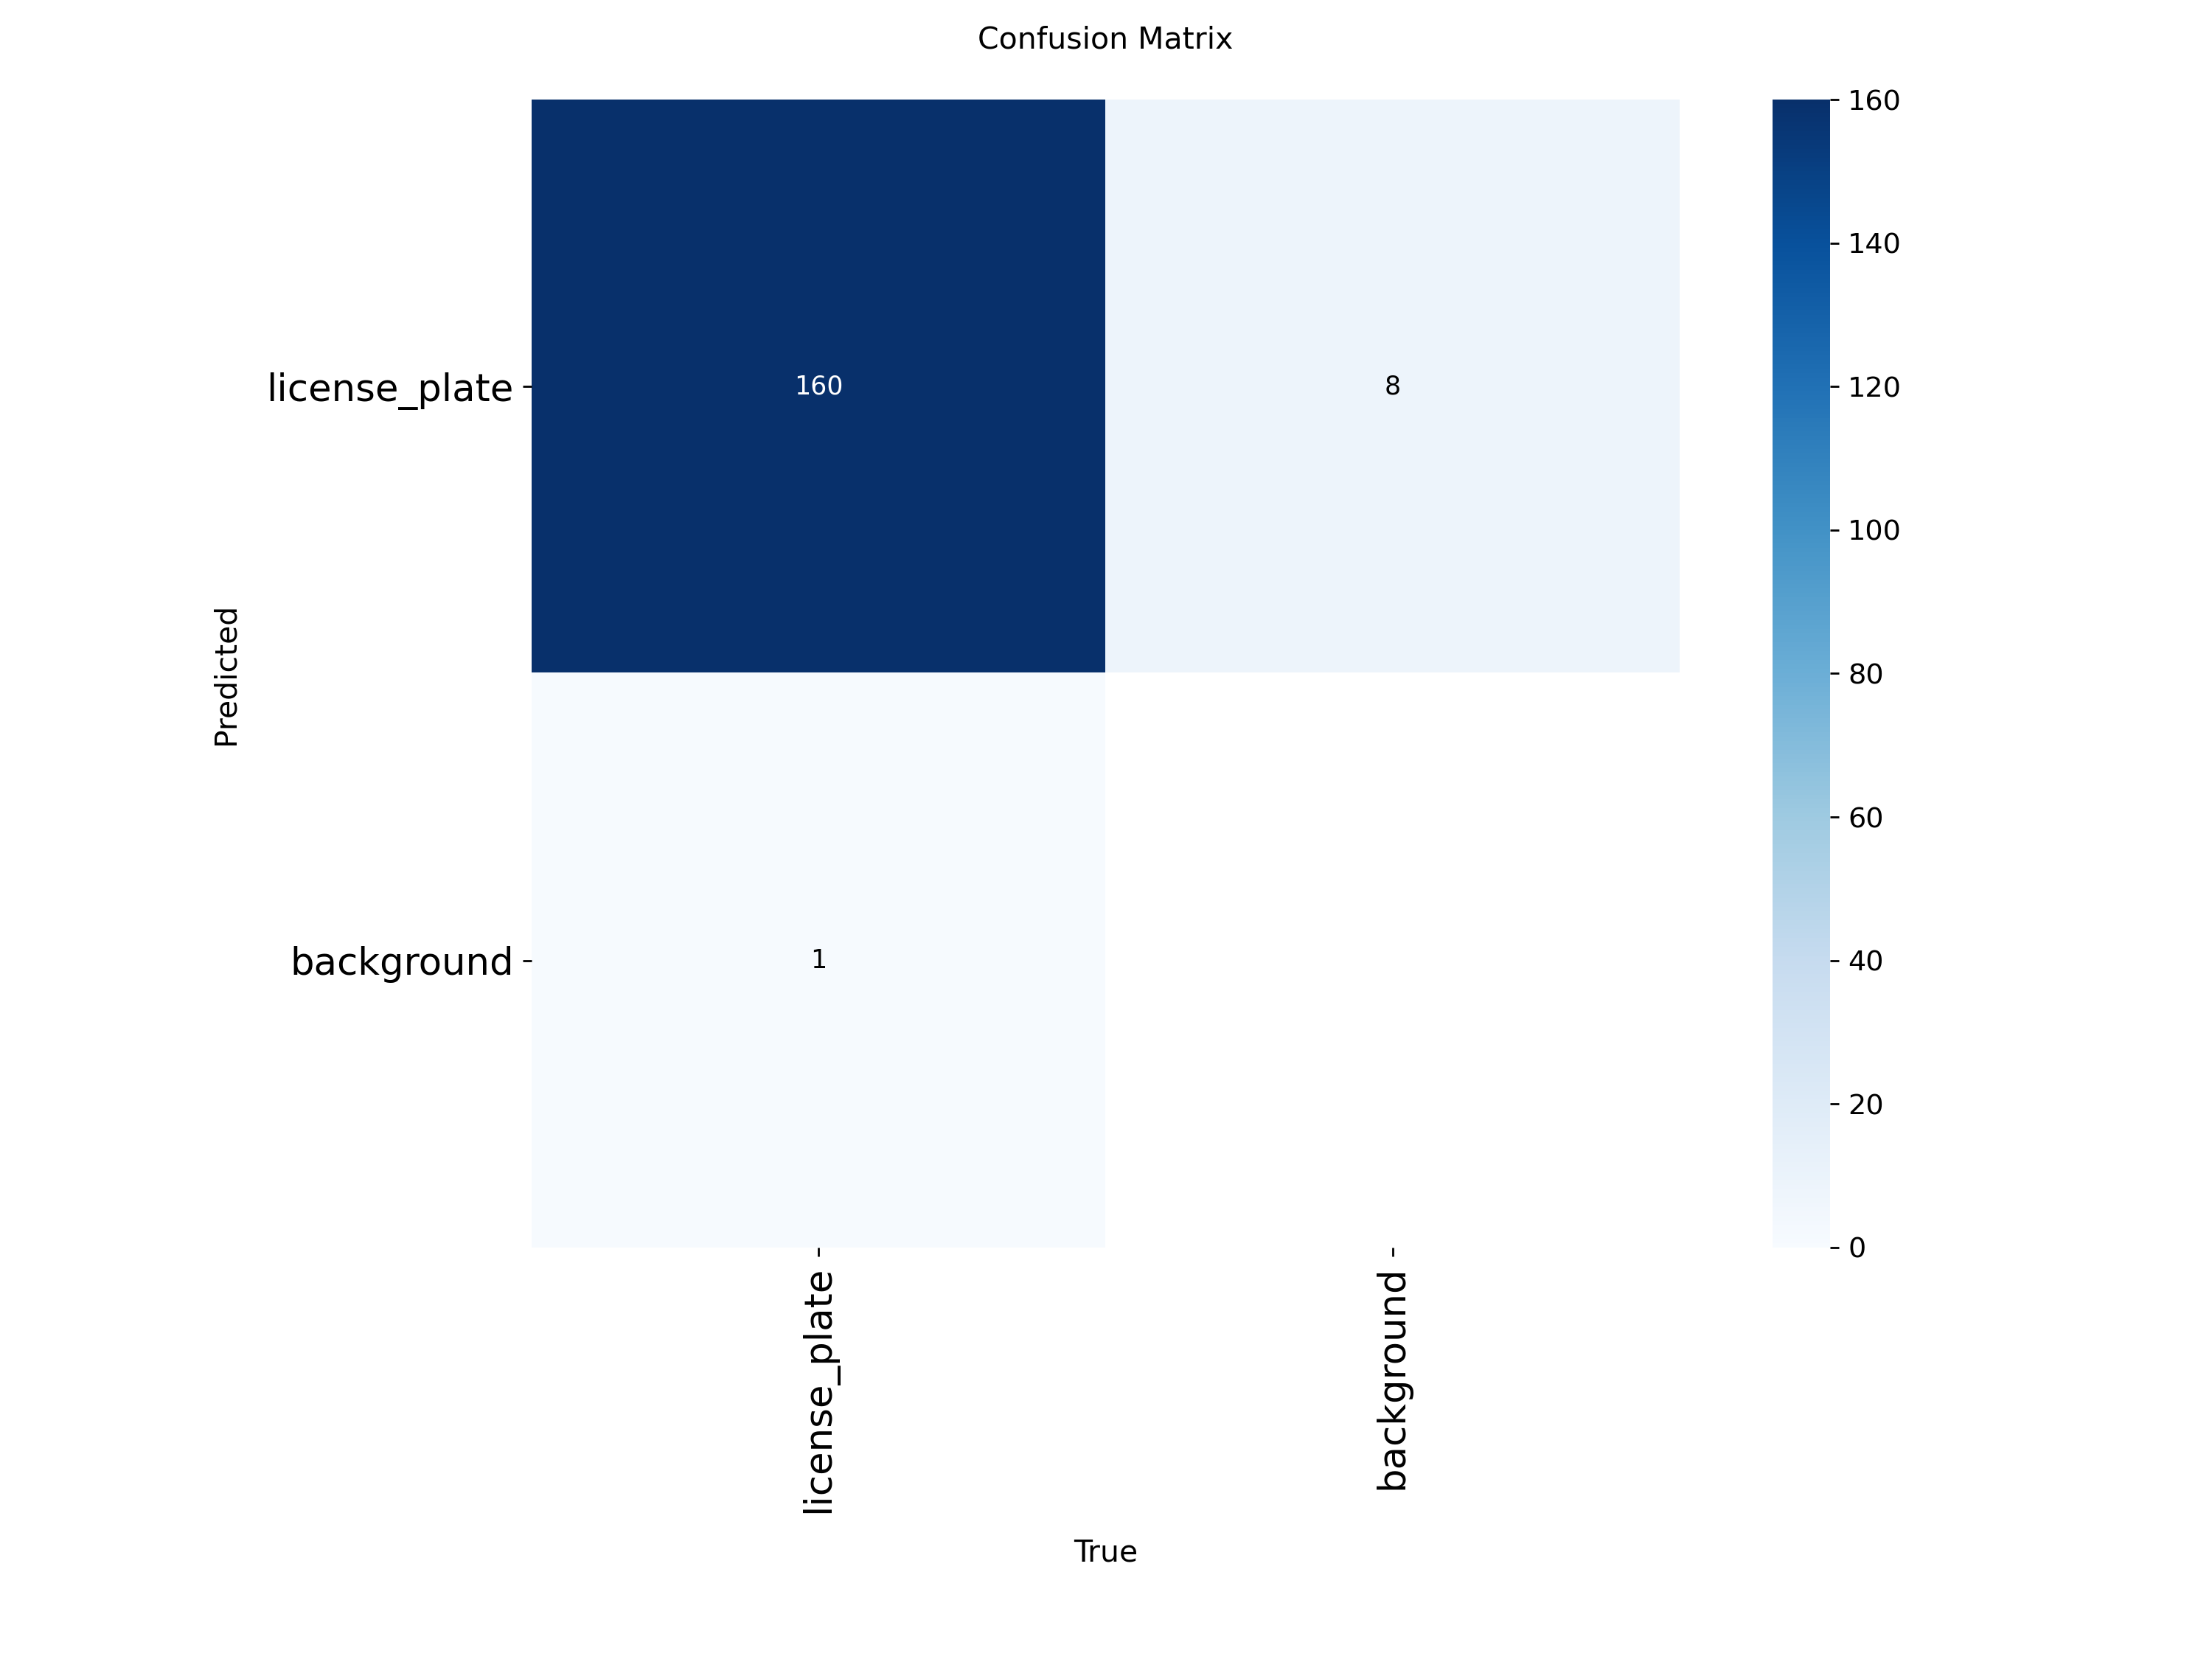
\includegraphics[width=\textwidth]{fig/proy/confusion_matrix-new-model.png}
	\caption{Matriz de confusión del mejor modelo de detección de placas}
	\label{fig:mejor-modelo-yolo}
\end{figure}

En este capítulo se exponen los diseños experimentales realizados para
comprobar el funcionamiento correcto del sistema. Por ejemplo, si se
realiza algún sistema con reconocimiento de patrones, usualmente esta
sección involucra las llamadas \emph{matrices de confusión} donde se
compactan las estadísticas de reconocimiento alcanzadas. En circuitos
de hardware, experimentos para determinar variaciones contra ruido,
etc. También pueden ilustrarse algunos resultados concretos como
ejemplo del funcionamiento de los algoritmos. Puede mostrar por medio
de experimentos ventajas, desventajas, desempeño de su algoritmo, o
comparaciones con otros algoritmos.

Recuerde que debe minimizar los ``saltos'' que el lector deba hacer en
su documento. Por tanto, usualmente el análisis se coloca junto a
\tablas y figuras presentadas, y debe tener un orden de tal modo que se
observe cómo los objetivos específicos y el objetivo general del
proyecto de tesis se han cumplido.
